\chapter{Resultados}

En este capítulo se muestra una aplicación

Todos los cálculos aquí expuestos fueron realizados a través del lenguaje y entorno de programación orientado a la estadística, \texttt{R} (R core team, 2017).


\section{Determinación del rango de cointegración y estimación del modelo lineal de corrección del error}

En este apartado se utiliza principalmente el paquete \texttt{vars} (Pfaff, 2008). 

Antes de la determinación del rango de cointegración del proceso, es necesario tener en cuenta que el uso del contraste de cointegración de Johansen que se utilizará para dichos fines es sensible a la especificación del modelo vectorial de corrección del equilibrio que subyace. Para la especificación de dicho modelo se recurrió a diferentes criterios. 

De manera similar a como señalan Ben Kaabia \& Gil (2008), se observa que al realizar los contrastes univariantes de raíz unitaria, no se rechaza la existencia de una raíz unitaria en torno a una constante no nula. Así también, al realizar los mismos contrastes para las series en primeras diferencias, estas resultaron estacionarias. Por último, en términos económicos, la presencia de una constante indica que existe una diferencia de escala entre los precios mayoristas y detallistas. 

El número de rezagos a incluir en el modelo se determinó con el objetivo de prevenir problemas de autocorrelación. De esta manera, se estimó el modelo secuencialmente utilizando entre 2 y  12 rezagos y se calculó el estadístico de Ljung-Box multivariado para los residuos rezagados entre el orden mínimo posible y aquellos de orden 52. Los p-valores correspondientes a cada uno de los contrastes están resumidos en la figura \ref{fig5.6}. De esta manera, se aprecia que la hipótesis nula de independencia no se puede rechazar a un nivel de significancia de 5\% en la mayoría de los casos para el modelo con siete términos rezagados. 

\begin{figure}
\centering
\caption{Contrastes de Ljung-Box para diferentes especificaciones del modelo}
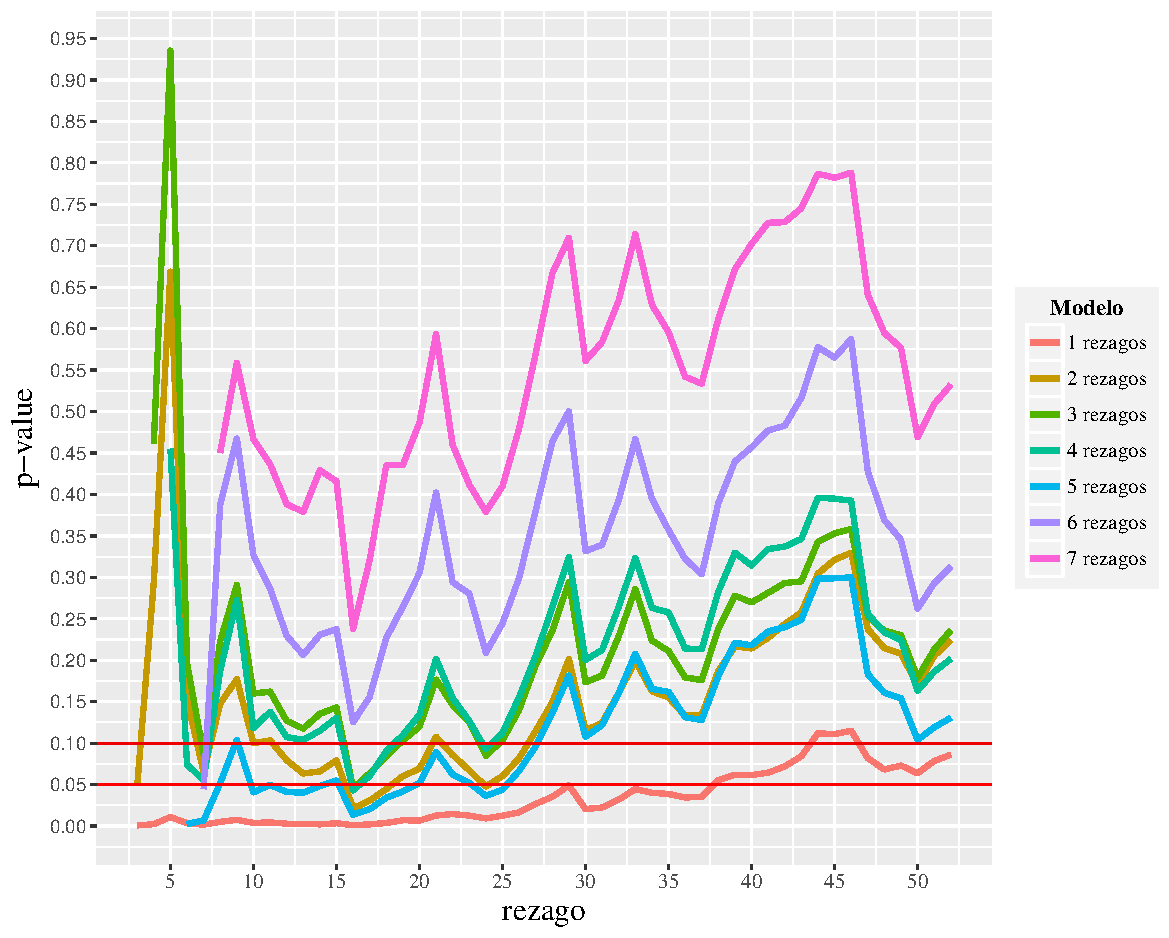
\includegraphics[scale=0.6]{fig_results/fig1.pdf}
\floatfoot{Fuente: Elaboración propia}
\end{figure}


De esta forma, el modelo definitivo a estimar resultó ser el siguiente: 

\begin{equation}
\Delta \mathbf{y}_{t} = \boldsymbol{\Pi}\mathbf{y}_{t-1}+\sum_{i=1}^{7}\boldsymbol{\Gamma_{i}}\mathbf{y}_{t-i}+\boldsymbol{\varepsilon}_{t}
\end{equation}

Definido el número de rezagos a utilizar y la estructura del vector cointegrante, se procedió a aplicar el contraste de cointegración de Johansen, cuyos resultados pueden apreciarse en los cuadros \ref{tab5.15} y \ref{tab5.16}

\begin{table}[!htpb]
\caption{Contraste de la \textit{la traza} de cointegración de Johansen\label{tab5.15}}
\begin{center}
\begin{tabular}{@{}lrllll@{}}
\toprule
\multicolumn{1}{l}{} & \multicolumn{2}{c}{Estadístico} &
\multicolumn{3}{c}{Valores críticos} \\
\cmidrule(l){2-3} \cmidrule(l){4-6} \\
\multicolumn{1}{l}{$\mathcal{H}_0$} & \multicolumn{2}{c}{$p = 7$} &
\multicolumn{1}{l}{90\%}&
\multicolumn{1}{l}{95\%}&
\multicolumn{1}{l}{99\%}
\\
\midrule
$r \leq 1$  & \multicolumn{2}{c}{5.01}  & 7.52 & 9.24 & 12.97\\
$r = 0$     & \multicolumn{2}{c}{ 37.85}  & 17.85 & 19.96 & 24.60\\
\bottomrule
\end{tabular}
\end{center}
\label{tab-10}
\end{table}

En el cuadro \ref{tab5.15} se observa el rechazo de la hipótesis $\mathcal{H}_{0}: = 0$ lo que descarta que la especificación adecuada sea un modelo VAR en niveles. Por otro lado, la hipótesis nula $\mathcal{H}_{0}\leq 1$ no puede rechazarse. 


\begin{table}[!htpb]
\caption{Contraste del \textit{máximo autovalor} de cointegración de Johansen\label{tab5.16}}
\begin{center}
\begin{tabular}{@{}lrllll@{}}
\toprule
\multicolumn{1}{l}{} & \multicolumn{2}{c}{Estadístico} & \multicolumn{3}{c}{Valores críticos} \\
\cmidrule(l){2-3} \cmidrule(l){4-6} \\
\multicolumn{1}{l}{$\mathcal{H}_0$} & \multicolumn{2}{c}{$p = 8$} &
\multicolumn{1}{l}{90\%}&
\multicolumn{1}{l}{95\%}&
\multicolumn{1}{l}{99\%}
\\
\midrule
$r \leq 1$ & \multicolumn{2}{c}{5.01} & 7.52 & 9.24 & 12.97 \\
$r = 0$ & \multicolumn{2}{c}{32.84} & 13.75 & 15.67 & 20.20 \\
\bottomrule
\end{tabular}
\end{center}
\label{tab-11}
\end{table}

Al realizar la prueba de acuerdo al máximo autovalor, se observa el mismo resultado. 

De esta manera, el modelo puede especificarse como 

\begin{equation}
 \Delta\mathbf{y}_{t} = \boldsymbol{\alpha \beta}^{'}\left[\begin{array}{c}1 \\ \mathbf{y}_{t-1}\end{array}\right]+\sum_{i=1}^{8}\boldsymbol{\Gamma}_{i}\Delta\mathbf{y}_{t-i}+\boldsymbol{\varepsilon}_{t}
\end{equation}

Donde $\boldsymbol{\alpha}=\left[\begin{array}{c} \alpha_{1} \\ \alpha_{2} \end{array}\right]$ y $\boldsymbol{\beta}^{'} = \left[\begin{array}{ccc} \frac{\beta_{0}}{\beta_{2}} & 1 & \frac{\beta_{3}}{\beta_{2}} \end{array}\right]$

Teniendo en cuenta que para ser identificado el vector cointegrante debe estar normalizado. El modelo finalmente a estimar es: 

\begin{equation}
\begin{array}{c} \Delta y_{1t} \\ \Delta y_{2t} \end{array} = 
\begin{array}{c} \alpha_{1}(\beta^{*}_{0}+y_{1t}+\beta^{*}_{1}y_{2t}) \\
                       \alpha_{2}(\beta^{*}_{0}+y_{1t}+\beta^{*}_{1}y_{2t})\end{array}+
\begin{array}{c} \sum_{i}^{7}\phi_{11,i}\Delta y_{1t-i}+\sum_{i}^{7}\phi_{12,i}\Delta y_{2t-i} \\
                 \sum_{i}^{7}\phi_{21,i}\Delta y_{1t-i}+\sum_{i}^{7}\phi_{22,i}\Delta y_{2t-i}\end{array}+
                 \begin{array}{c} \varepsilon_{1t} \\ \varepsilon_{2t} \end{array}
\end{equation}

Donde $\beta_{0}^{*}=\frac{\beta_{1}}{\beta_{2}}$ y $\beta_{1}^{*}=\frac{\beta_3}{\beta_{2}}$.

\begin{table}[!htpb]
\centering
\begin{threeparttable}
\caption{Modelo de corrección hacia el equilibrio (\textbf{VECM}) estimado mediante método de máxima verosimilitud \label{vecm_f}}
\begin{tabular}{@{}lll@{}}
\toprule
\multicolumn{3}{c}{Vector cointegrante} \\
\midrule 
Mayoristas & Supermercados & constante \\ 
1             & -1.087 & 0.987 \\
\midrule
 & $\Delta \text{Mayoristas}_{t} $ & $\Delta \text{Supermercados}_{t}$ \\ 
 \midrule 
\text{Corrección del error} & -0.138(0.029)*** & 0.023(0.015) \\
$\Delta$mayorista$_{t-1}$ & 0.2(0.049)*** & 0.071(0.026)*** \\
$\Delta$mayorista$_{t-2}$ & 0.062(0.051)** & 0.088(0.027) \\
$\Delta$mayorista$_{t-3}$ & 0.033(0.05) & 0.04(0.026)*** \\
$\Delta$mayorista$_{t-4}$ & -0.047(0.049)* & 0.022(0.026) \\
$\Delta$mayorista$_{t-5}$ & -0.038(0.049) & -0.029(0.026) \\
$\Delta$mayorista$_{t-6}$ & 0.07(0.049) & 0.043(0.026) \\
$\Delta$mayorista$_{t-7}$ & 0.019(0.049) & 0.074(0.026) \\
$\Delta$supermercado$_{t-1}$ & 0.205(0.089) & -0.072(0.047)* \\
$\Delta$supermercado$_{t-2}$ & 0.158(0.089) & -0.018(0.047) \\
$\Delta$supermercado$_{t-3}$ & 0.05(0.089) & 0.037(0.047) \\
$\Delta$supermercado$_{t-4}$ & 0.08(0.088) & 0.083(0.046)* \\
$\Delta$supermercado$_{t-5}$ & 0.021(0.087) & -0.032(0.046) \\
$\Delta$supermercado$_{t-6}$ & 0.03(0.085) & 0.014(0.045)*** \\
$\Delta$supermercado$_{t-7}$ & 0.186(0.083)** & -0.019(0.044) \\
\midrule 
AIC & BIC & SSR \\ 
\midrule 
-5465.432 & -5335.279 & 4.425978 \\
\bottomrule
\end{tabular}
\begin{tablenotes}
\small 
\item $^{a}$: Errores estándar entre paréntesis. 
\item $^{b}$: significativo a: * 10\%, **5\%, *** 1\%
\end{tablenotes}
\end{threeparttable}
\end{table}



De los resultados provistos en el cuadro (\ref{vecm_f}) se desprende que la elasticidad de largo plazo de los precios de supermercados con respecto a los precios mayoristas es de aproximadamente 0.92, lo que indica un comportamiento relativamente inelástico. Es decir, cuando los mayoristas suben el precio en 1\% los supermercados lo hacen en un orden de 0.92\%. Esto contradice la hipótesis de transmisión perfecta de precios, en cuyo caso, el valor de la elasticidad debiera ser 1. Debido a esto a continuación se estima el modelo restringido, para determinar la evidencia estadística en favor o en contra de esta hipótesis, de la siguiente forma, utilizando una matriz $\mathbf{H}$ que permite incorporar las restricciones sobre el modelo: 

\begin{equation}
\mathbf{H}\boldsymbol{\beta} = \left[\begin{array}{ccc} 1 & -1 & 0 \\ 
                                                            0 &  0 &  1 \end{array}\right]
                                   \left[\begin{array}{c} 
                                    \beta_{1} \\ \beta_{2} \\ \beta_{3} \end{array}\right]=\begin{array}{c} 0 \\ 0 \end{array}
\end{equation}


\begin{table}[!htpb]
\centering
\begin{threeparttable}
\caption{Contraste de homogeneidad en precios \label{blrtest}}
\begin{tabular}{@{}llll@{}}
\toprule \\
Hipótesis & Estadístico & Grados de libertad & p-value \\
\midrule 
$\mathcal{H}_{0}:\beta_{2}=\beta_{3}=1$ & 0.8798 & 1 & 0.35
\\
\bottomrule
\end{tabular}
\end{threeparttable}
\end{table}

Del resultado del contraste de razón de verosimilitud expuesto en el cuadro (\ref{blrtest}) se tiene que no se puede rechazar la hipótesis acerca de que la transmisión es perfecta en el largo plazo. Esto significa que la relación cointegrante puede reescribirse de la siguiente forma: 

\begin{equation}
\log P_{t}^{c} = 0.3305+\log P_{t}^{p}
\end{equation}

A continuación se presentan los resultados para el modelo restringido 


\begin{table}[!htpb]
\centering
\begin{threeparttable}
\caption{Modelo de corrección hacia el equilibrio (\textbf{VECM}) restringido \label{vecm_rest}}
\begin{tabular}{@{}lll@{}}
\toprule
\multicolumn{3}{c}{Vector cointegrante} \\
\midrule 
Mayoristas & Supermercados & constante \\ 
1             & -1 & -0.3304581 \\
\midrule
 & $\Delta \text{Mayoristas}_{t} $ & $\Delta \text{Supermercados}_{t}$ \\ 
 \midrule 
 $\text{corrección del error}$ &  0.13300 (0.02752)***    & -0.01489 (0.01449)  \\     
$\Delta$supermercados$_{t-1} $ & -0.07855 (0.04675)**  &  0.21312 (0.08876)*    \\   
$\Delta$mayoristas$_{t-1}    $ &    0.19365 (0.04825)*** &   0.07725 (0.02541).     \\  
$\Delta$supermercados$_{t-2} $ & 0.16574 (0.08865).    &  -0.02221 (0.04669)   \\   
$\Delta$mayoristas$_{t-2}    $ &  0.05746 (0.04988) & 0.09346 (0.02627)***   \\     
$\Delta$supermercados$_{t-3} $ &  0.05759 (0.08892)    &  0.04480 (0.02615)  \\
$\Delta$mayoristas$_{t-3}    $ &  0.02912 (0.04965)   & 0.04480 (0.02615).     \\   
$\Delta$supermercados$_{t-4} $ &  0.08859 (0.08744)   & 0.02675 (0.04605).   \\     
$\Delta$mayoristas$_{t-4}    $ & -0.05076 (0.04882)    &  -0.05076 (0.02675)  \\   
$\Delta$supermercados$_{t-5} $ & 0.03105 (0.08690)    & -0.03430 (0.04577)   \\     
$\Delta$mayoristas$_{t-5}    $ & -0.04163 (0.04860)    &  -0.02537 (0.02560)  \\   
$\Delta$supermercados$_{t-6} $ &  0.03908 (0.08473)    &  0.01272 (0.04463)  \\     
$\Delta$mayoristas$_{t-6}    $ &  0.06732 (0.04836)   & 0.04671 (0.02547).   \\     
$\Delta$supermercados$_{t-7} $ & 0.19470 (0.08318)*    &  -0.01940 (0.04381)  \\     
$\Delta$mayoristas$_{t-7}    $ &  0.01660 (0.04842)  &  0.07771 (0.02550)**   \\   
\bottomrule
\end{tabular}
\begin{tablenotes}
\small 
\item $^{a}$: Errores estándar entre paréntesis. 
\item $^{b}$: significativo al: . 10\%, *5\%, ** 1\%, ***0.1\%
\end{tablenotes}
\end{threeparttable}
\end{table}

Con lo que utilizando el resultado expuesto en la ecuación (\ref{margen}), se puede afirmar que el margen que los supermercados mantienen en el largo plazo es de 39\%. Un resultado ligeramente superior al que se obtendría como el promedio de las diferencias entre los logaritmos de los precios, que corresponde a 32.64\%. Además de los resultados del cuadro (\ref{vecm_rest}), se confirma que existe un comportamiento de corrección hacia el equilibrio, pues cuando dicho término tiene variaciones positivas, los mayoristas responden bajandos sus precios. Así también, cabe mencionar que la relación con el término corrección del error es significativa para el caso de los mayoristas, pero no así para los supermercados. Esto se puede inferir a raíz de que en el modelo de \textbf{VECM} todas las variables explicativas son estacionarias, por lo que el uso del contraste $t$ es válido en muestras grandes. 

De todas formas, se procedió a aplicar un contraste de razón de verosimilitud para deteminar la hipótesis de exogeneidad débil. 



Aunque varios de los coeficientes representantes de la dinámica de corto plazo en el cuadro (\ref{vecm_rest}) son significativos, su interpretación no es directa, pues el modelo por construcción presenta problemas de multicolineadad. Para analizar la respuesta del sistema frente a diferentes perturbaciones, se utilizan las funciones de impulso respuesta, como se señala en el capítulo 3. 



\begin{figure}[H]
\centering
\caption{Función de impulso respuesta: Impulso desde el precio mayorista}
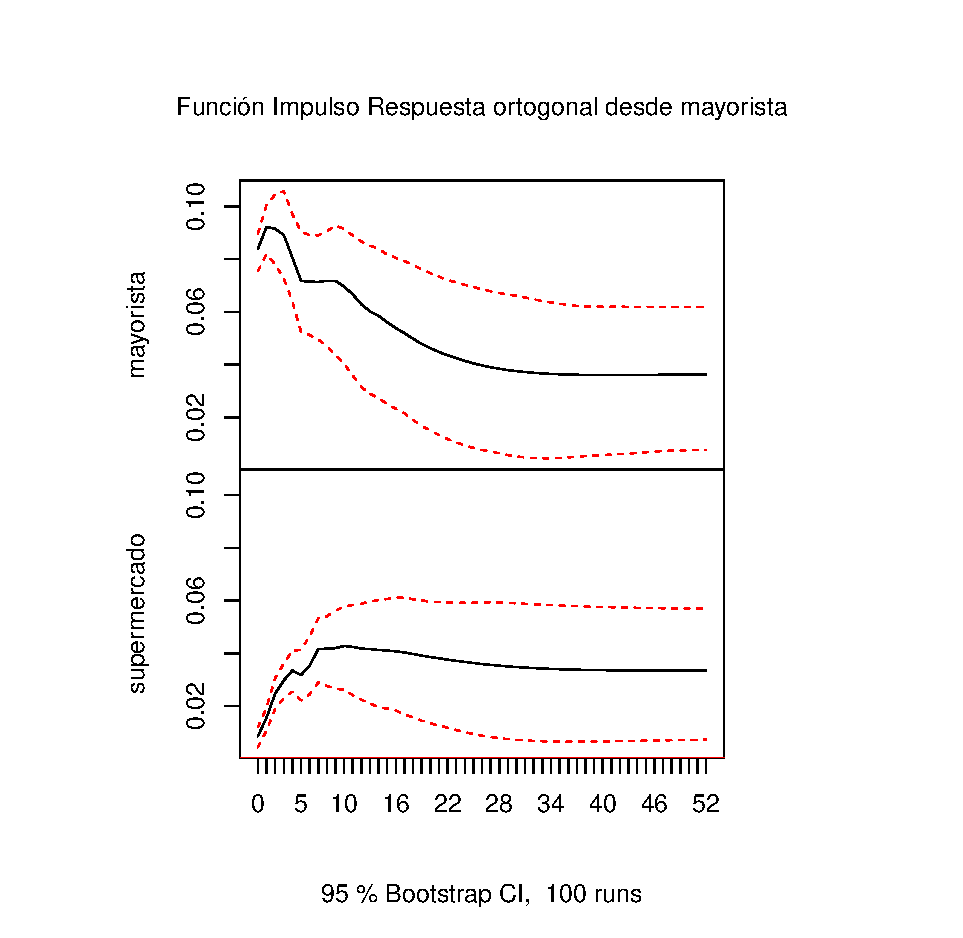
\includegraphics[scale=0.7]{fig_results/fig2.pdf}
\floatfoot{Fuente: Elaboración propia}
\end{figure}

\begin{figure}[H]
\centering
\caption{Función de impulso respuesta: Impulso desde el precio de supermercados}
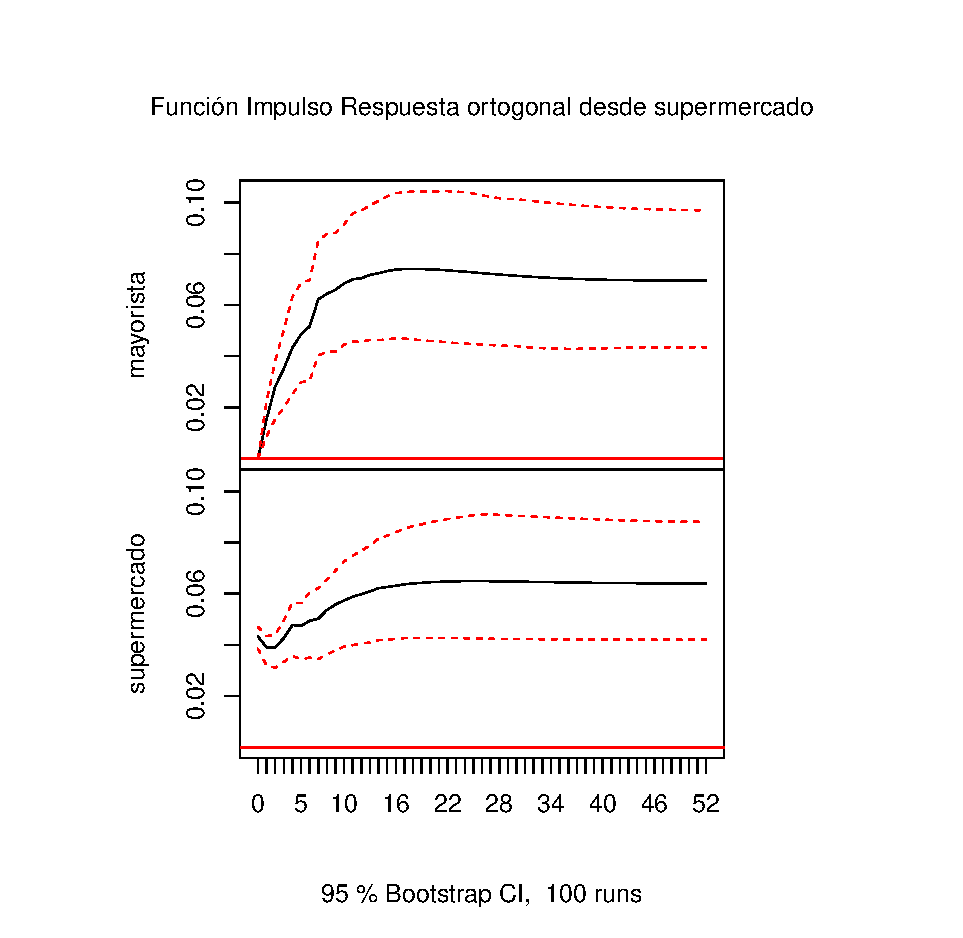
\includegraphics[scale=0.7]{fig_results/fig3.pdf}
\floatfoot{Fuente: Elaboración propia}
\end{figure}

\section{Diagnósticos del modelo lineal}

\begin{figure}[H]
\centering
\caption{Residuos del modelo lineal}
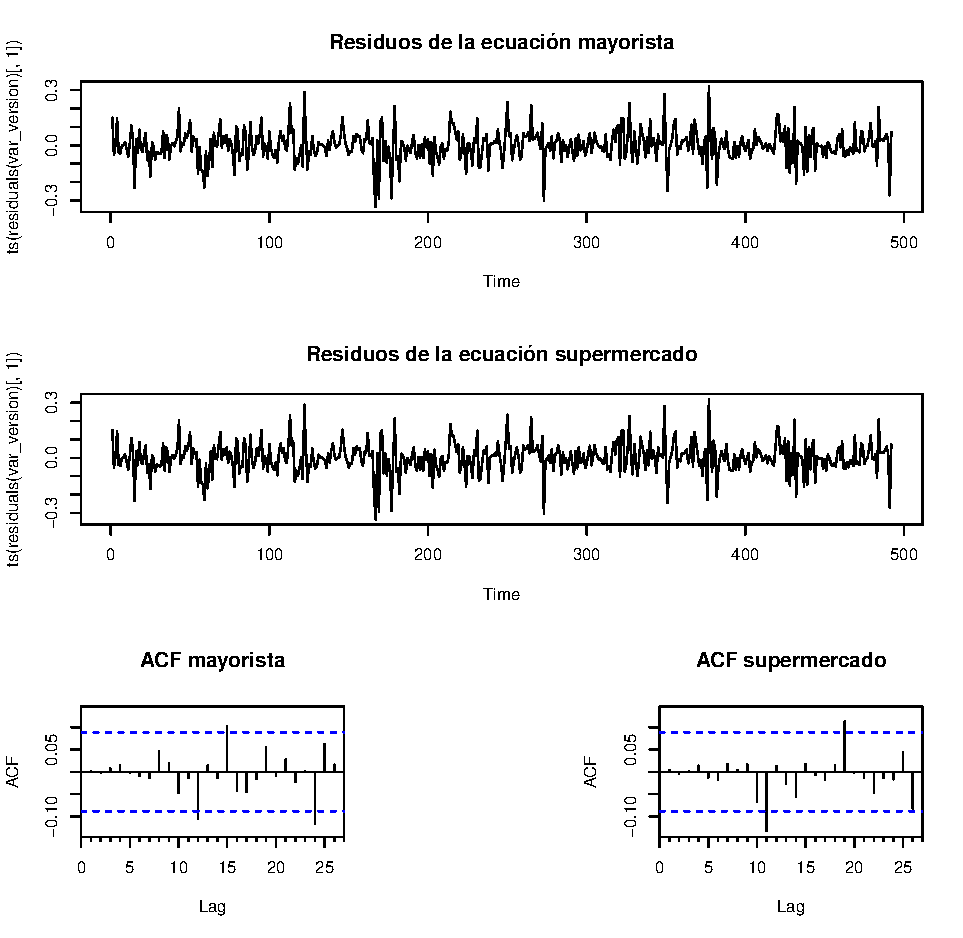
\includegraphics[scale=0.7]{fig_results/fig4.pdf}
\floatfoot{Fuente: Elaboración propia}
\end{figure}

\begin{figure}[H]
\centering
\caption{Histograma bivariado de los residuos}
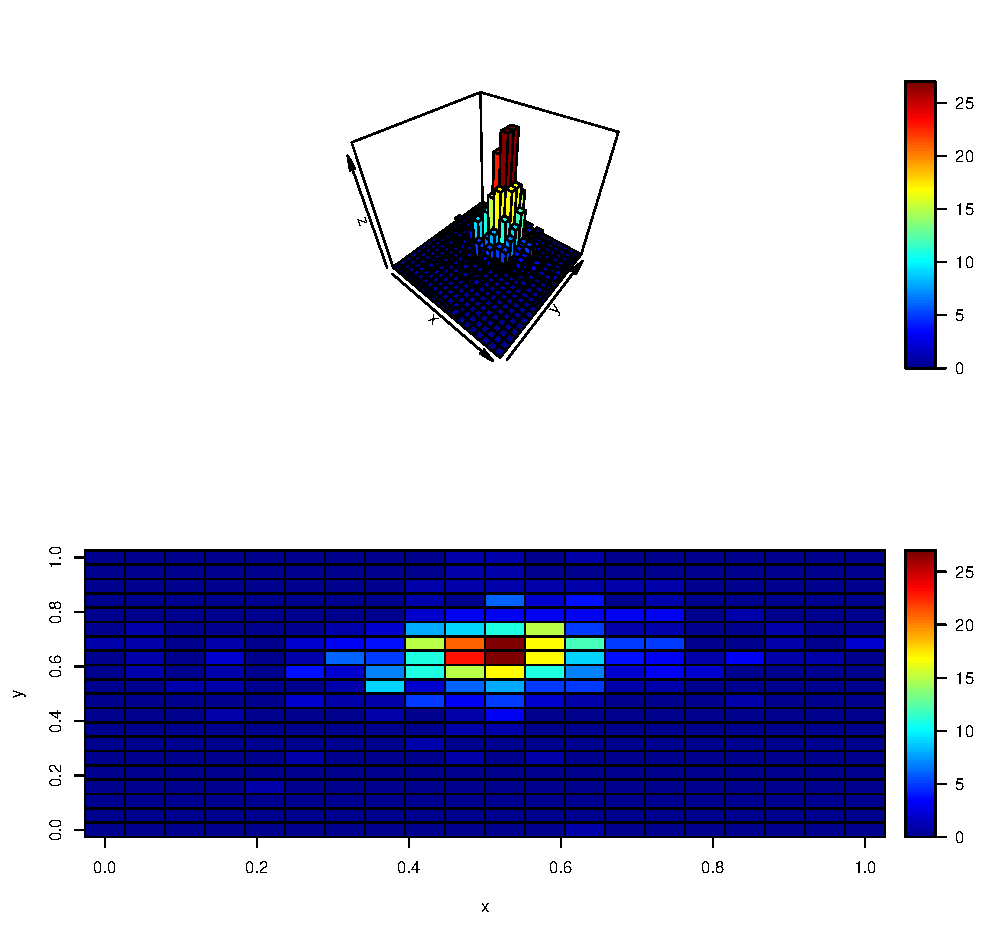
\includegraphics[scale=0.7]{fig_results/fig5.pdf}
\floatfoot{Fuente: Elaboración propia}
\end{figure}


\begin{table}[!htpb]
\centering
\caption{Diagnósticos del modelo}
\begin{tabular}{@{}llll@{}}
\toprule \\ 
Contraste   & $E$ & df & $\mathbb{P}(\chi^{2}>E)$ \\
\midrule \\ 
Doornik \& Hansen & 246.913 & 4 & 2.11$\times 10^{-45}$ \\
Jarque-Bera (Multivariado) & 30.141 & 4 & $<$2.85$\times 10^{-7}$ \\
ARCH (Multivariado) & 144.4 & 81 & 1.89$\times 10^{-5}$ \\ 
\bottomrule 
\end{tabular}
\end{table}

\section{Estimación del modelo vectorial de corrección del error por umbrales \textbf{TVECM}}
Los contrastes y estimaciones de esta sección fueron realizadas a través del paquete \texttt{tsDyn} de Di Narzo, Aznarte \& Stigler(2009).

El paquete \texttt{tsDyn} y la función asociada a este, \texttt{TVECM.HStest}, no permiten utilizar una constante en la relación de cointegración, por lo que para esto se debió modificar ligeramente el código original de la función recién mencionada, pues como ha sido descrito en el capítulo 3, la estimación del modelo VECM se construye sobre la base de un modelo lineal, por lo que sólo bastó con incorporar la constante en la estimación del primer paso a través de una nueva función denominada \texttt{TVECM\_HStest2}. 

\begin{figure}[H]
\centering
\caption{Contraste de Hansen \& Seo (2002)}
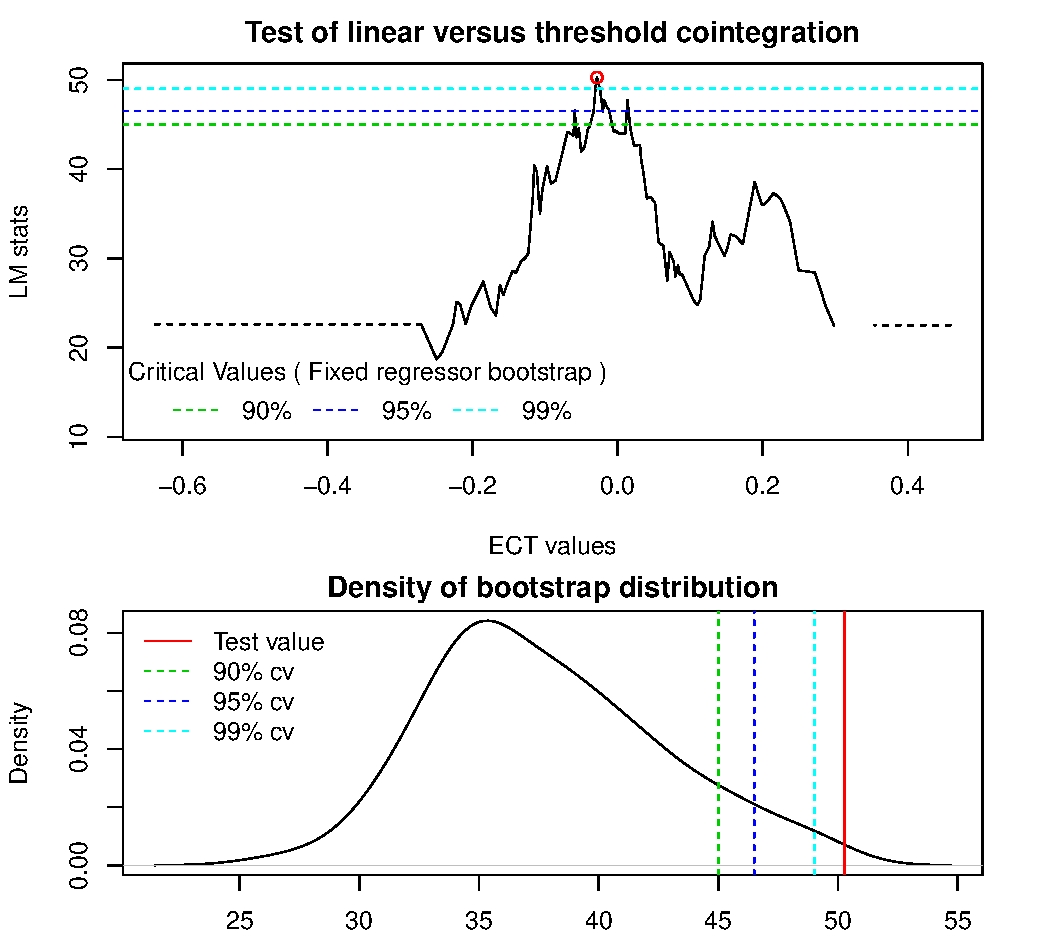
\includegraphics[scale=0.7]{fig_results/fig6.pdf}
\floatfoot{Fuente: Elaboración propia}
\end{figure}

\begin{table}[H]
\centering
\caption{Contraste de Hansen \& Seo 2002}
\begin{tabular}{@{}lll@{}}
\toprule \\ 
\multicolumn{2}{c}{Estadístico} & P-Value \\
\midrule \\ 
\multicolumn{2}{c}{50.27302}  & 0 \\
\bottomrule 
\multicolumn{3}{c}{Valores críticos} \\
10\% & 5\% & 1\% \\
\midrule
45.00837 & 46.50572 & 49.02173 \\
\bottomrule 
\multicolumn{3}{c}{Vector cointegrante} \\
\midrule 
Mayoristas & Supermercados & constante \\ 
1             & -1.087 & 0.987 \\
\bottomrule 
\bottomrule
\end{tabular}
\floatfoot{Fuente: Elaboración propia}
\end{table}


\begin{figure}[H]
\centering
\caption{Estimación del modelo TVECM. Búsqueda simultánea de $\beta$ y $\gamma$}
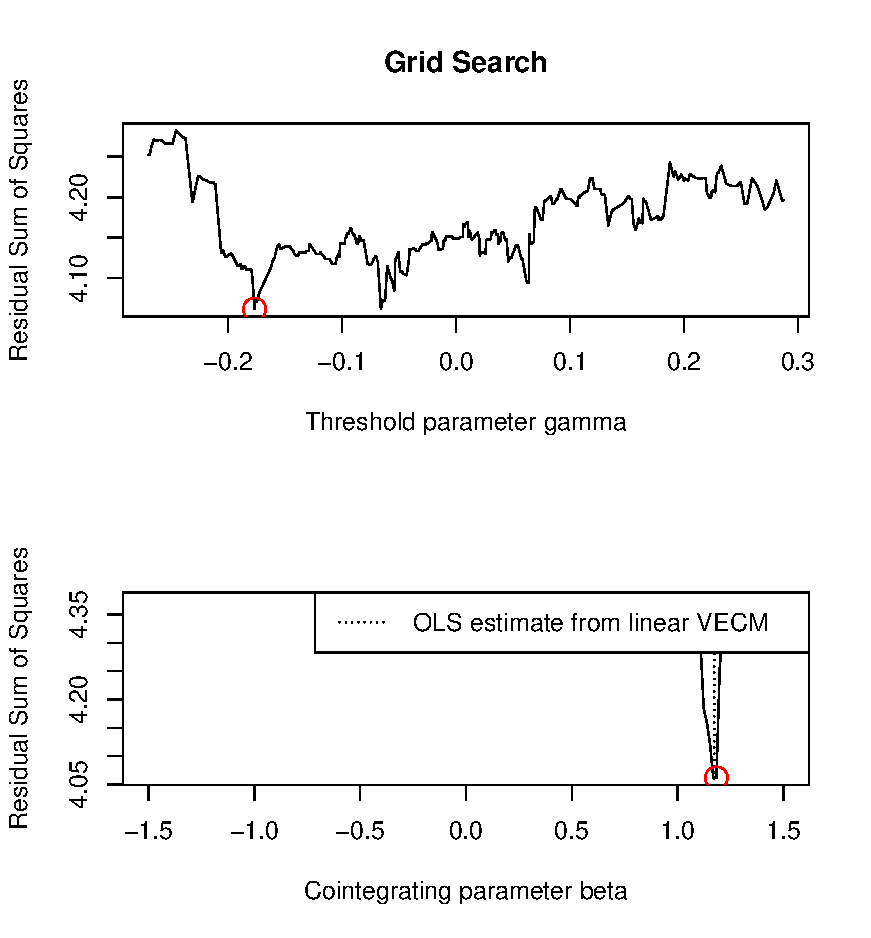
\includegraphics[scale=0.7]{fig_results/fig7.pdf}
\floatfoot{Fuente: Elaboración propia}
\end{figure}


\begin{table}[H]
\centering
\caption{Modelo TVECM sin restringir}
\begin{tabular}{@{}lll@{}}
\toprule \\
\multicolumn{3}{c}{Vector cointegrante} \\
\midrule 
Mayoristas & Supermercados & constante \\ 
1             & -1.1834 & - \\
\midrule
 & $\Delta$mayoristas & $\Delta$supermercados \\ 
\midrule 
\multicolumn{3}{c}{$\gamma<-0.177$} \\
\midrule 
corrección del error & -0.023 (0.033) &0.036 (0.017)* \\
$\Delta$mayorista$_{t -1}$ & -0.06 (0.092) &-0.017 (0.048) \\
$\Delta$supermercado$_{t -1}$ & 0.501 (0.166)** &0.121 (0.086) \\
$\Delta$mayorista$_{t -2}$ & 0.053 (0.09) &-0.004 (0.047) \\
$\Delta$supermercado$_{t -2}$ & 0.516 (0.173)** &-0.035 (0.09) \\
$\Delta$mayorista$_{t -3}$ & -0.009 (0.085) &0.001 (0.044) \\
$\Delta$supermercado$_{t -3}$ & -0.174 (0.147) &0.158 (0.076) \\
$\Delta$mayorista$_{t -4}$ & -0.169 (0.084)* &0.081 (0.044). \\
$\Delta$supermercado$_{t -4}$ & 0.012 (0.168) &0.343 (0.087)*** \\
$\Delta$mayorista$_{t -5}$ & 0 (0.078) &-0.056 (0.04) \\
$\Delta$supermercado$_{t -5}$ & 0.076 (0.189) &-0.064 (0.099) \\
$\Delta$mayorista$_{t -6}$ & -0.128 (0.081) &-0.018 (0.042) \\
$\Delta$supermercado$_{t -6}$ & 0.275 (0.176) &0.159 (0.092). \\
$\Delta$mayorista$_{t -7}$ & -0.051 (0.078) &0.112 (0.04) \\
$\Delta$supermercado$_{t -7}$ & 0.517 (0.151)*** &-0.014 (0.079) \\
\midrule 
\multicolumn{3}{c}{$\gamma\geq -0.177$} \\
\midrule 
corrección del error & -0.209 (0.044)*** &-0.017 (0.023) \\
$\Delta$mayorista$_{t -1}$ & 0.288 (0.056)*** &0.12 (0.029)*** \\
$\Delta$supermercado$_{t -1}$ & 0.081 (0.107) &-0.135 (0.056)* \\
$\Delta$mayorista$_{t -2}$ & 0.031 (0.059) &0.147 (0.031)*** \\
$\Delta$supermercado$_{t -2}$ & 0.024 (0.104) &-0.013 (0.054) \\
$\Delta$mayorista$_{t -3}$ & 0.063 (0.06) &0.085 (0.031)** \\
$\Delta$supermercado$_{t -3}$ & 0.143 (0.113) &-0.054 (0.059) \\
$\Delta$mayorista$_{t -4}$ & 0.032 (0.059) &-0.004 (0.031) \\
$\Delta$supermercado$_{t -4}$ & 0.1 (0.102) &-0.027 (0.053) \\
$\Delta$mayorista$_{t -5}$ & -0.11 (0.062). &-0.005 (0.032) \\
$\Delta$supermercado$_{t -5}$ & 0.012 (0.098) &-0.024 (0.051) \\
$\Delta$mayorista$_{t -6}$ & 0.148 (0.06)* & 0.076 (0.031)* \\
$\Delta$supermercado$_{t -6}$ & -0.069 (0.096) &-0.015 (0.05) \\
$\Delta$mayorista$_{t -7}$ & 0.043 (0.061) &0.069 (0.032)* \\
$\Delta$supermercado$_{t -7}$ & 0.054 (0.099) &-0.007 (0.051) \\
\midrule 
\multicolumn{3}{c}{Porcentaje de observaciones en cada regimen 27\% y 73\%}  \\
 \bottomrule \\ 
\bottomrule
\end{tabular}
\floatfoot{Fuente: Elaboración propia}
\end{table}

\begin{figure}[H]
\centering
\caption{Estimación del modelo TVECM Restringido. Búsqueda de $\gamma$}
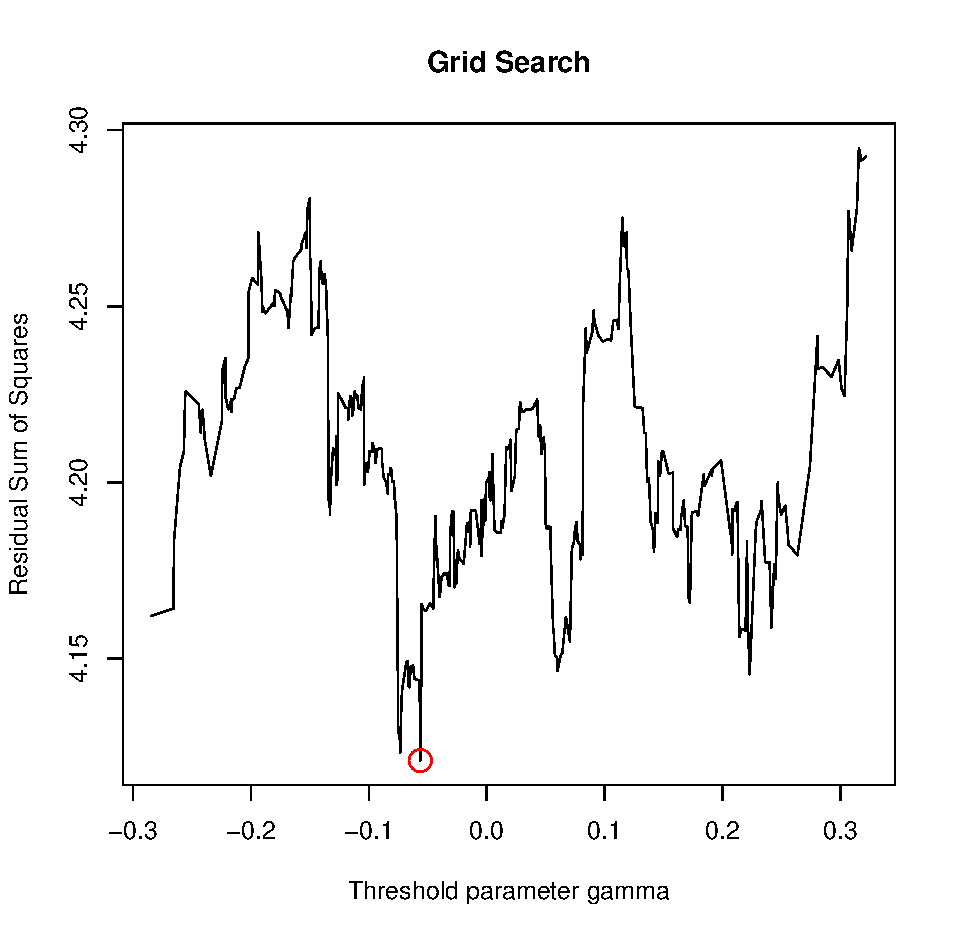
\includegraphics[scale=0.7]{fig_results/fig8.pdf}
\floatfoot{Fuente: Elaboración propia}
\end{figure}


\begin{table}[H]
\centering
\caption{Modelo TVECM sin restringir}
\begin{tabular}{@{}lll@{}}
\toprule \\
\multicolumn{3}{c}{Vector cointegrante} \\
\midrule 
Mayoristas & Supermercados & constante \\ 
1             & -1 & 0.3305 \\
\midrule
 & $\Delta$mayoristas & $\Delta$supermercados \\ 
\midrule 
\multicolumn{3}{c}{$\gamma<-0.0563156$} \\
\midrule 
Corrección del error & -0.06 (0.044) & 0.056 (0.023) \\
$\Delta$mayorista$_{t-1}$ & 0.025 (0.086) & 0.013 (0.045) \\
$\Delta$supermercado$_{t-1}$ & 0.327 (0.137) & -0.045 (0.072) \\
$\Delta$mayorista$_{t-2}$ & 0.019 (0.082) & 0.005 (0.043) \\
$\Delta$supermercado$_{t-2}$ & 0.332 (0.124) & -0.084 (0.065) \\
$\Delta$mayorista$_{t-3}$ & -0.049 (0.08) & -0.001 (0.042) \\
$\Delta$supermercado$_{t-3}$ & -0.082 (0.127) & 0.12 (0.066) \\
$\Delta$mayorista$_{t-4}$ & -0.134 (0.075) & 0.078 (0.039) \\
$\Delta$supermercado$_{t-4}$ & 0.006 (0.12) & 0.196 (0.063) \\
$\Delta$mayorista$_{t-5}$ & 0.035 (0.074) & -0.035 (0.039) \\
$\Delta$supermercado$_{t-5}$ & -0.071 (0.133) & -0.088 (0.069) \\
$\Delta$mayorista$_{t-6}$ & -0.022 (0.072) & 0.031 (0.038) \\
$\Delta$supermercado$_{t-6}$ & 0.17 (0.118) & 0.044 (0.062) \\
$\Delta$mayorista$_{t-7}$ & -0.075 (0.069) & 0.076 (0.036) \\
$\Delta$supermercado$_{t-7}$ & 0.308 (0.126) & -0.039 (0.066) \\
\midrule 
\multicolumn{3}{c}{$\gamma\geq -0.0563156$} \\
\midrule 
Corrección del error & -0.167 (0.035) & -0.011 (0.018) \\
$\Delta$mayorista$_{t-1}$ & 0.269 (0.058) & 0.103 (0.03) \\
$\Delta$supermercado$_{t-1}$ & 0.126 (0.116) & -0.101 (0.061) \\
$\Delta$mayorista$_{t-2}$ & 0.074 (0.063) & 0.144 (0.033) \\
$\Delta$supermercado$_{t-2}$ & -0.072 (0.129) & 0.078 (0.067) \\
$\Delta$mayorista$_{t-3}$ & 0.09 (0.063) & 0.08 (0.033) \\
$\Delta$supermercado$_{t-3}$ & 0.17 (0.126) & -0.058 (0.066) \\
$\Delta$mayorista$_{t-4}$ & 0.036 (0.064) & -0.025 (0.034) \\
$\Delta$supermercado$_{t-4}$ & 0.195 (0.127) & -0.056 (0.066) \\
$\Delta$mayorista$_{t-5}$ & -0.11 (0.064) & -0.006 (0.033) \\
$\Delta$supermercado$_{t-5}$ & 0.11 (0.114) & 0.006 (0.059) \\
$\Delta$mayorista$_{t-6}$ & 0.137 (0.065) & 0.056 (0.034) \\
$\Delta$supermercado$_{t-6}$ & -0.205 (0.127) & -0.012 (0.067) \\
$\Delta$mayorista$_{t-7}$ & 0.088 (0.067) & 0.079 (0.035) \\
$\Delta$supermercado$_{t-7}$ & 0.159 (0.11) & 0.001 (0.057) \\
\midrule 
\multicolumn{3}{c}{Porcentaje de observaciones en cada regimen 40.66\% y 59.34\%}  \\
 \bottomrule \\ 
\bottomrule
\end{tabular}
\floatfoot{Fuente: Elaboración propia}
\end{table}


\section{Diagnósticos del modelo no lineal}








